\section{Drogon -- The Robot Simulator}
{
    \subsection{Introduction}
     
    To effectively analyze and verify the proposed solutions, a real robot was needed. Unfortunately with the COVID-19 situation, making a real robot became almost impossible with all the supply shortages and supply chain disturbances. Simulating the manipulator becomes the second option in this case. Although its not a definitive answer but with careful assumptions, a simulator ca very well be used to verify the proposals.

    On a lighter note, just like the name Gregor, \textbf{Drogon} was also taken from a fictional character in one of the George R. R. Martin's Game of thrones novels; a mighty dragon.

    \subsubsection{The Requirements}
    Another problem was finding the best simulator to carry out the task. With no earlier training in simulators but a years of experience in programming, I decided to program an in-vitro simulator. The simulator was required to posses some important features and requirements.

    \textbf{The Simulator:}
    \begin{itemize}
      \item Simulate the position and links of the manipulator in discrete time domain.
      \item Simulate the output motors and actuators
      \item PID controllers
      \item Simulate the effect of gravity
      \item Angular and linear momentum
    \end{itemize}

    \textbf{Analysis Tools:}
    \begin{itemize}
      \item $3$~D visualizer
      \item Plotting
      \item Workspace optimizer
      \item Export data for further analysis
      \item Path planner
      \item Manual motor control
      \item Manual end effector control
      \item Machine codes parser
    \end{itemize}

    Out of all these features, there were some that could not be completed or had to be skipped given the scope of the work. Since one may be very tempted to code them or even use them, the doors to implement them are open in the code. The features are as following:
    \begin{itemize}
      \item PID controller (partly implemented)
      \item Linear and angular momentum (partly implemented)
      \item Machine code parser
    \end{itemize}

    Comprehensiveness is the core attribute of Drogon. It provides, under one screen, the flexibility to introduce an elementary change in the design, like, the maximum speed of an actuator and directly observe the consequences on all of the analysis tools. One can choose to programmatically or manually signal an actuator to move in a particular direction and position, and visualize the outcome in a $3$D preview window. It also integrates with Gregor to support the live editing and visualization of rotating bezier spline curves

    Besides comprehensiveness, our design tool offers a set of powerful analysis tools which enabled us to solve complex robot maneuvers and optimize the solution. Performing mechanical simulation with simplified real world constraints, $3$D live preview of the moving robot, work-space optimizer, $2$D art drawing, investigating the actuator velocity in continuous and discrete demain are some of the tools we used for optimization in our design.

    Since the tool is based on in-vitro coding, it can be taught to easily integrate with and inside Microcontrollers to practically , Proteus and SolidEdge to give more design flexibility.

    \subsection{The working principal}
    In this section we discuss the working principals of different aspects of the simulator.

    \subsubsection{Simulation}
    The simulator used in this work is designed from scratch. It is highly customizable in terms of coding and usage. In one configuration it can simulate a manipulator based on steppers motors. This way, the complexity of implementing the effect of gravitational and reactional forces on each actuator. In another configuration, it can simulate actuators with a limited output power, torque/force, response time and even a feedback mechanism making them essentially servo actuators. Not all of the actuators have to this way and the governing limits can also be changed at run-time. Just like the first one, in this configuration too, it first uses forward kinematics of the robot to find out the required position of its actuators to achieve a particular end-effector position and orientation. Unlike stepper motors that can just take a required number of steps in a limited time to achieve a certain position regardless of the load it has to carry, for a servo actuator, the simulator has to calculate the gravitational loads on individual links and propagate the forces and torques to individual actuator. The controller of the actuator is, in parallel, deciding how much output it must produce. Once the simulator has both the forces on each joint, it can calculate the accelerations. And once the accelerations are calculated, it only needs to be integrated with each \emph{tick} of the simulator to yield velocity and position of the actuator. At this point, it may become quite clear that implementing the gyroscopic effects of the links become quite a challenge. Since the robot being analyzed is not supposed to be working at high speeds and loads, the error caused by ignoring this effect in approximation would be negligible.

    \subsubsection{Motor controller}
    One can choose to use either a stepper motor or a DC servo on every joint. In case of stepper motors, one can configure:
    \begin{itemize}
      \item number of steps per revolution, and
      \item minimum step time.
    \end{itemize}
    In this case the simulator assumes:
    \begin{itemize}
      \item the step time remains the same regardless of the motor speed, and
      \item the motor can take a step regardless of the applied load.
    \end{itemize}
    While in case of a servo motor one can configure:
    \begin{itemize}
      \item the maximum input electrical power,
      \item the maximum torque,
      \item maximum idle acceleration,
      \item maximum velocity, and
      \item the \emph{P}, \emph{I} and \emph{D} parameters of the controller.
    \end{itemize}
    In this case, the simulator assumes that:
    \begin{itemize}
      \item the motor are $100$~% energy efficient,
      \item they are weightless, as in they are installed in the base of the robot with mechanical links transferring the power through the arm,
      \item at a constant power, the torque reduces inversely with speed ($Power = torque \times speed$), and
      \item the PID controllers operate independently.
    \end{itemize}

    Moreover, the PID controllers work on a very simple equation
    Later on, it was discovered that implementing simple PID controllers that take the required position as reference were not very effective. So the actuators are kept as stepper motors by default and can be changed to servo motors. Work is still needed to either fine tune the PID controllers or even run them on a more powerful controller.

    More details on the working principles of the simulator will be discussed in later chapters. Also, the installation and usage of the tool is described in detail in Appendix B.

    \subsubsection{Workspace}
    The workspace contains a spherical manipulator as discussed in chapter \ref{chapter2}. The simulator considers the robot fixed on a horizontal surface at the origin $(0, 0, 0)$ with the first link along the vertical axis.

    \subsection{About the Tools}

    An shape independent model of the robot under simulation can be visualized in real time using ``$3D$ Animation'' tool as seen in Fig. \ref{Fig3D}. The ``Robot Feet Position'' tool gives a superior insight on the stability of the robot. It can be seen in Fig. 1A(e) that the center of gravity plot can help optimize the motion where stability is a concern. Using the trajectory of the center of the robot in the global frame of reference can help determine the most efficient actuator movements which can be used to displace the robot from a specific position. Screen shots of the plot produced using the ``Top Trajectory'' tool can be seen in Fig. 1A(d).


        \begin{figure}
          \centering
          \includegraphics[width=0.7\textwidth]{3D.png}
          \caption{A screenshot of the $3$D representation tool. The blue sphere under the end effector shows the target given to the robot.
          } \label{Fig3D}
        \end{figure}

    All of the tools can output in real time. The robot configuration and other parameters change with time, producing animations which make it easier to decipher the underlying information.

    \subsection{Workspace Optimization}
    The workspace optimizer allows to simulate the robot solution recursively through discrete sections of the defined workspace and evaluates the degrees of freedom the robot has  specific parts of the workspace. It then colors the segments to give a more clear idea of the robot workspace. The user can then modify the robot and see, in-result, the change in the workspace. A typical output of the workspace is show in Fig.

        \begin{figure}
          \centering
          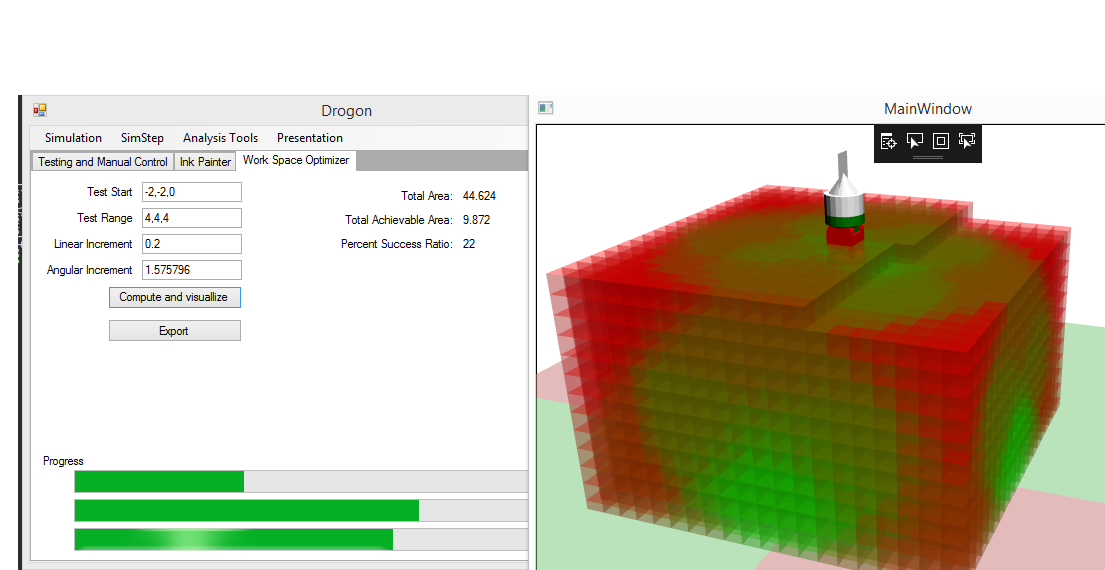
\includegraphics[width=0.9\textwidth]{WorkSpaceOptimer.png}
          \caption{The workspace is coded in colors. Purely green blocks represent a point where the robot has all of the degrees of freedom and the slightly red blocks indicate the parts where robot starts to loose one or more degrees of freedom.
          } \label{FigWorkspace}
        \end{figure}
    \subsection{Script Path Planner}
    As already mentioned, I've included a tool to construct bezier rotation splines in the tool which can serialize the data in computer files and also load from existing files. A screenshot can be seen in Fig.

        \begin{figure}
          \centering
          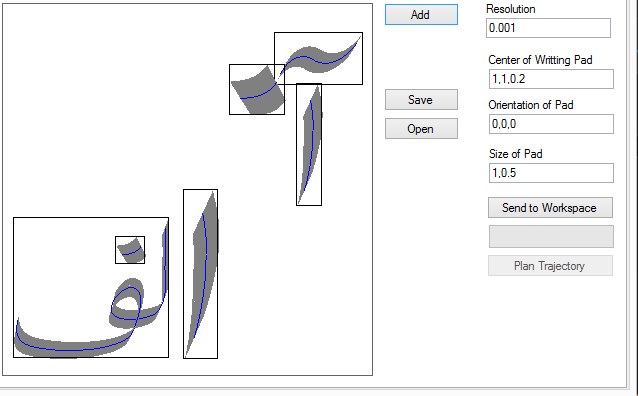
\includegraphics[width=0.9\textwidth]{SctiptEditor.png}
          \caption{The script maker can manage multiple splines and render robot trajectory according to the user resolution requirement.
          } \label{FigWorkspace}
        \end{figure}
    \subsection{Script Motion Simulator}
    Once the script is constructed using the script maker, it can be transported to the workspace in any orientation. The robot then plans how to make the required maneuvers and sibilates the behaviour. A screenshot of a robot writting a script can be seen in figure \ref{FigScriptMotion}
        \begin{figure}
          \centering
          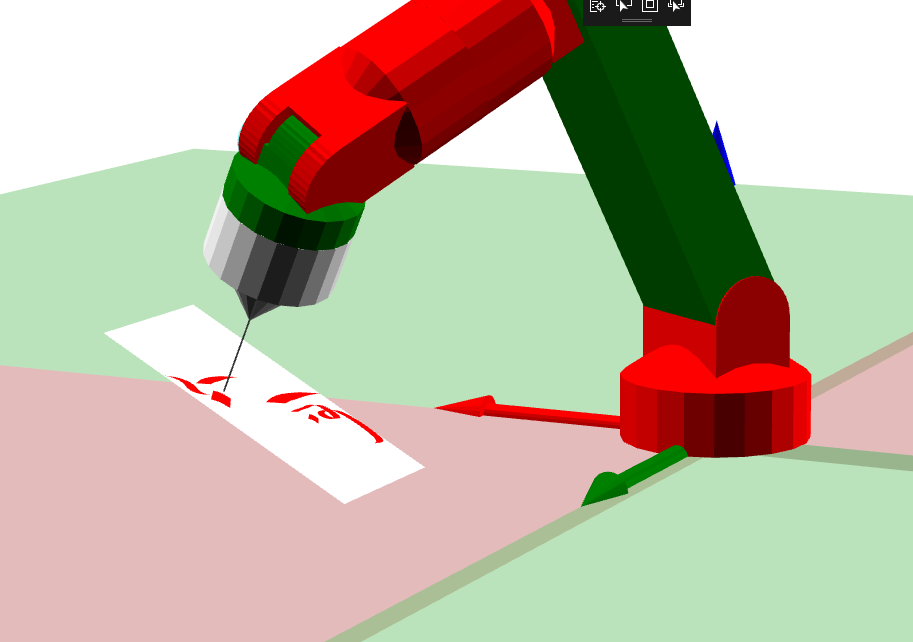
\includegraphics[width=0.9\textwidth]{writting.PNG}
          \caption{Robot writting on a slanted plane.
          } \label{FigScriptMotion}
        \end{figure}
}
\subsection{Requirements and Features}
\subsection{3D Visualizer}
\subsection{Workspace Optimizer}
\subsection{PID Tuner}
\subsection{Rotating Spline Importer}
\subsection{Usage}
\subsection{Interface}
\subsubsection{Manual Control}
\subsubsection{Analysis Tools}
\subsection{Development}
\subsubsection{Code Organization}
\subsubsection{The SphericalRobot Class}
\subsection{Simulation}
\subsubsection{Assumptions and Limitations}
\subsubsection{Accuracy of simulated Quantities}
\subsubsection{Forward Kinematics}
\subsubsection{Rotating Bezier Spline Curves}
\subsection{Sample Results}
\subsubsection{Accuracy}
\subsection{Areas that Need Improvement}
